\documentclass{beamer}

\usetheme{Warsaw}
\usefonttheme[onlylarge]{structurebold}
\setbeamerfont*{frametitle}{size=\normalsize,series=\bfseries}
\setbeamertemplate{navigation symbols}{}

\usepackage[english]{babel}
\usepackage[utf8]{inputenc}
\usepackage{times}
\usepackage[T1]{fontenc}
\usepackage{changepage}

\title{Django Channels\\Introduction}
\author[rwar]{Radoslaw Warzocha}
%\date{I dont know the date yet}

\begin{document}

\begin{frame}
	\titlepage
\end{frame}

\section{Motivation}

\begin{frame}{Motivation}
	\begin{center}
		Django is awesome\\
		\vspace{1em}
		But it's also \textit{request} based and bound to \textit{pull/get} model\\
		\vspace{1em}
		More and more often we need to use\\
		\textit{server push} technology
	\end{center}
\end{frame}

\begin{frame}{Motivation}
	\begin{adjustwidth}{2em}{2.5em}
	\begin{itemize}
		\item WebSockets
		\item HTTP long polling
		\item HTTP2 push
		\item Extendability to other protocols\\ (e.g. WebRTC, raw UDP, SMS)
	\end{itemize}
	\end{adjustwidth}
\end{frame}

\begin{frame}{HTTP2 utilization}
	\begin{center}
		\begin{figure}
			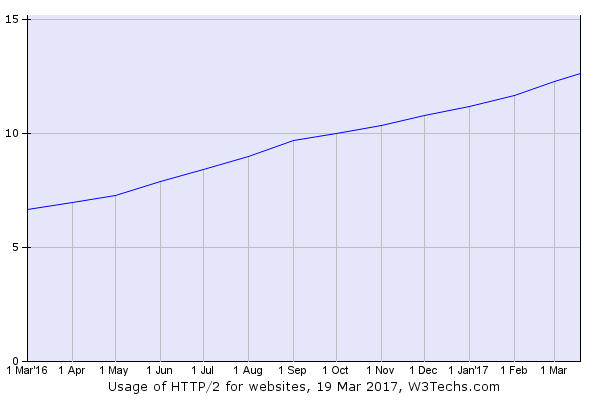
\includegraphics[scale=0.45]{ce-http2.png}
		\end{figure}
	\end{center}
\end{frame}

\section{Core concepts}

\begin{frame}{Core concepts}
	\begin{adjustwidth}{2em}{2.5em}
	\begin{itemize}
		\item Channel
			\begin{itemize}
				\item FIFO
				\item message expiry
				\item at-most-once delivery
			\end{itemize}
		\item Groups
	\end{itemize}
	\end{adjustwidth}
\end{frame}

\begin{frame}{Core concepts}
	\begin{adjustwidth}{2em}{2.5em}
	\begin{itemize}
		\item ASGI
		\item Consumers
		\item Routing
	\end{itemize}
	\end{adjustwidth}
\end{frame}

\section{Examples}

\subsection{Running the application}

\section{Further reading}

\end{document}
